\documentclass{article}%
\usepackage[T1]{fontenc}%
\usepackage[utf8]{inputenc}%
\usepackage{lmodern}%
\usepackage{textcomp}%
\usepackage{lastpage}%
\usepackage[head=40pt,margin=0.5in,bottom=0.6in]{geometry}%
\usepackage{graphicx}%
%
\title{\textbf{Habitantes de Carabobo protestaron~por falta de gas doméstico}}%
\author{El Nacional Web}%
\date{06/12/2018}%
%
\begin{document}%
\normalsize%
\maketitle%
\textbf{URL: }%
http://www.el{-}nacional.com/noticias/protestas/habitantes{-}carabobo{-}protestaronpor{-}falta{-}gas{-}domestico\_262337\newline%
%
\textbf{Periodico: }%
EN, %
ID: %
262337, %
Seccion: %
Protestas\newline%
%
\textbf{Palabras Claves: }%
Carabobo, Protestas, Denuncia\newline%
%
\textbf{Derecho: }%
2.8, %
Otros Derechos: %
, %
Sub Derechos: %
2.8.1\newline%
%
\textbf{EP: }%
SI\newline%
\newline%
%
\textbf{\textit{Los residentes del municipio San Diego denunciaron que tienen más de dos meses sin recibir el servicio}}%
\newline%
\newline%
%
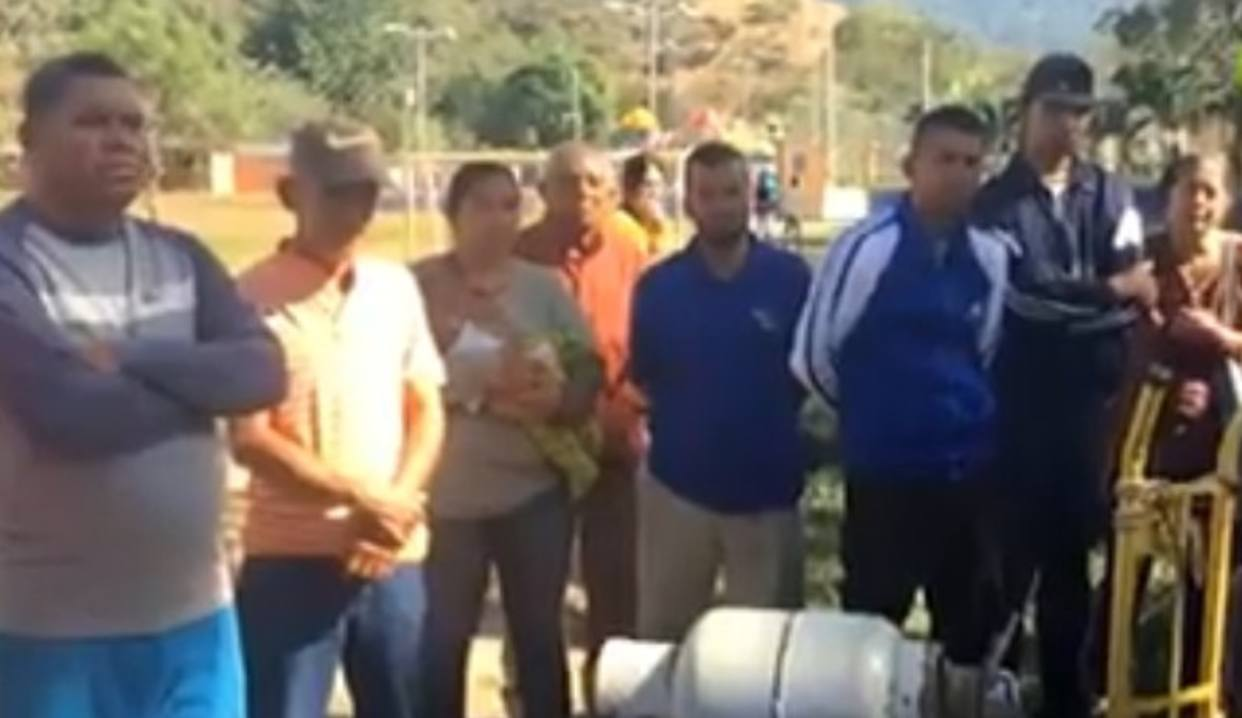
\includegraphics[width=300px]{89.jpg}%
\newline%
%
Vecinos del estado Carabobo protestaron este jueves por la falta de suministro de gas doméstico en el sector del municipio San Diego.%
\newline%
%
Los habitantes del municipio denunciaron que no cuentan con el suministro desde hace al menos dos meses y señalan que el camión que surte el gas no ha llegado a la localidad.%
\newline%
%
Agregaron que la situación los ha obligado a cocinar con leña, lo que afecta a los niños y a los adultos mayores que tienen problemas respiratorios.%
\newline%
%
En imágenes difundidas vía Twitter se puede observar que el grupo de personas estuvo~en el lugar con mensajes alusivos a su protesta.%
\newline%
%
\end{document}